\chapter{}

\section{Teori}
 Buat Resume Sejarah Python, perbedaan python 2 dan 3, dengan bahasa yang mudah dipahami dan dimengerti. Buatan sendiri bebas plagiat(10)
 
 Bahasa pemrograman Python dikembangkan oleh Guido van Rossum pada tahun 1990 di CWI, Amsterdam sebagai penerus dari bahasa pemrograman ABC. Versi terbaru yang dikeluarkan oleh pihak CWI adalah 1.2.

Pada ahun 1995, Guido melanjutkan pengembangan Python di CNRI. Versi terbarunya adalah 1.6. Pada tahun 2000, Guido dan team pengembang inti Python melakukan pengembangan di BeOpen.com,merupakan sebuah perusahaan komersial dan membentuk BeOpen PythonLabs. Lalu Python 2.0 dikeluarkan oleh BeOpen.

Pengembangan Python masih terus dilanjutkan dibawah arahan Guido dan Python Software Foundation. Python Software Foundation merupakan sebuah organisasi yang non-profit dibentuk untuk pemegang hak cipta intelektual Python dari versi 2.1 untuk mencegah Python dimiliki oleh perusahaan komersial lain. Saat ini pengembangan Python sudah sampai pada versi 2.6.1 dan versi 3.0.

Python juga memmiliki beberapa pembagian,yaitu paython 2 dan 3

\section{Resume Implementasi dan penggunaan Python di perusahaan dunia}
Didunia kerja sudah banyak developer yang menggunakan bahasa pemrograman python untuk perusahaannya diantaranya :
\begin{enumerate}
    \item 
    Netflix merupakan salah satu pengguna utama Python pada Central Alert Gateway. Aplikasi ini akan me-reroute alert dan mengirimkannya kepada individu atau kelompok yang berhak mengaksesnya.
    \item
    Instagram merupakan media sosial yang sangat populer pada saat ini. Dengan 400 juta pengguna aktif setiap harinya, tentu saja ini mematahkan pendapat banyak orang yang mengatakan bahwa aplikasi python tidak terlalu scalable. Menurut salah satu engineer di Instagram, moto para pengembang aplikasi di instagram adalah “Do the simple thing first,” dan hal ini sangat bisa dilakukan dengan menggunakan Python.
\end{enumerate}

\section{Instalansi Pyton 3}
\begin{enumerate}
    \item Tekan tombol kanan pada mouse lalu pilih open 

\begin{figure}[!htbp]
    \centering
    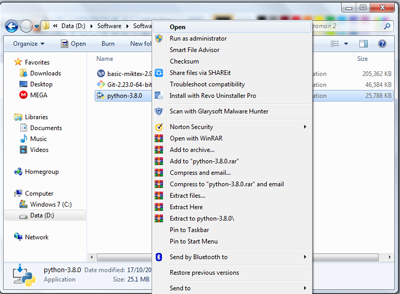
\includegraphics[scale=0.5]{figures/1.png}
    \label{visimisi}
\end{figure}

    \item Pilih Instal Now
    \begin{figure}[!htbp]
    \centering
    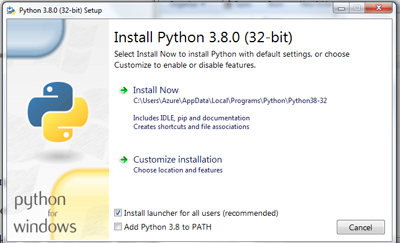
\includegraphics[scale=0.5]{figures/2.png}
    \label{visimisi}
\end{figure}


    \item Tunggu hingga instalansi selesai
    \begin{figure}[!htbp]
    \centering
    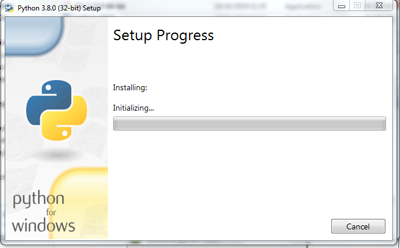
\includegraphics[scale=0.5]{figures/3.png}
    \label{visimisi}
\end{figure}
\end{enumerate}






\section{Instalasnsi Pip}
\begin{enumerate}
    \item Pertama Instal file get-pip.py dengan cara membuka file tersebut dengan Python.exe 
    
\begin{figure}[!htbp]
    \centering
    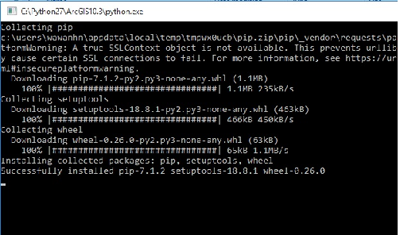
\includegraphics[scale=0.5]{figures/4.png}
    \label{visimisi}
\end{figure}

    \item Kedua set PATH dalam environmental variabel ke tempat dimana pip.exe berada

\begin{figure}[!htbp]
    \centering
    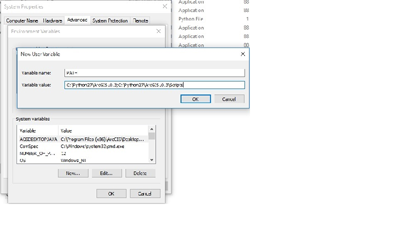
\includegraphics[scale=0.5]{figures/5.png}
    \label{visimisi}
\end{figure}

    \item ketiga  mengecek instalasi pip apakah berhasil dilakukan di komputer kita ketika perintah pip id command prompt.

\begin{figure}[!htbp]
    \centering
    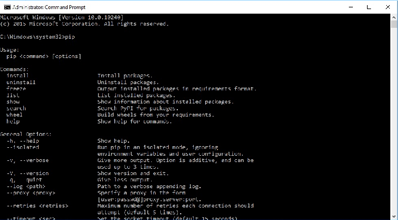
\includegraphics[scale=0.5]{figures/6.png}
    \label{visimisi}
\end{figure}
\end{enumerate}

\section{Menjalankan Script hello word di spyder}
\begin{enumerate}
    \item Buatlah scrip print ("Hellow World!")
\begin{figure}[!htbp]
    \centering
    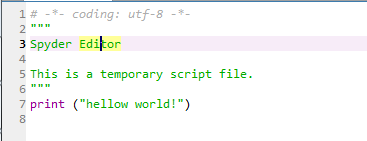
\includegraphics[scale=0.7]{figures/7.png}
    \label{visimisi}
\end{figure}

    \item Setelah selesai tekan lah tanda play 
\begin{figure}[!htbp]
    \centering
    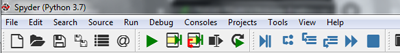
\includegraphics[scale=0.7]{figures/8.png}
    \label{visimisi}
\end{figure}
     \item Setelah itu akan keluar di consol Hellow World!
\end{enumerate}

\section{Penjelasan Identitas}
Operator identitas adalah operator yang memeriksa apakah dua buah nilai ( atau variabel ) berada pada lokasi memori yang sama. Operator biasa dikenal dengana nama identity operators.
Fungsi operator ini pada Python, dapat dibuat dengan kata kunci def dan nama fungsinya.
    def namafungsi():
    print "Hello ini Fungsi"
    
    Sama seperti blok kode yang lain, kita juga harus memberikan identasi (tab atau spasi 2x) untuk menuliskan isi fungsi.
Kita bisa manfaatkan parameter.

\section{Jenis jenis error identasi yang didapat}
\begin{enumerate}
    \item Run-time Error, kesalahan Run-time Error saat  kode program menjalankan perintah yang tidak logis. Contohnya jika kita menaruh sebuah file di directory 'C' lalu mengakses directory 'D'untuk mencari file yg kita simpan pada directory 'C' maka akan terjadi kesalahan alokasi directory.
    \item Syntax Error,Syntax Error terjadi apabila kita melakukan sebuah perintah atau statement yang diketik menyalahi aturan pengkodean oleh bahasa pemrograman yang digunakan. Semua bahasa pemrograman memiliki aturan pengkodean tersendiri.
    \item  Logical Error merupakan jenis kesalahan yang sulit dideteksi.Dikarena aplikasi yang mengalami Logical Error berjalan tanpa pesan kesalahan, tetapi menampilkan hasil yang tidak sesuai perintah.
\end{enumerate}
\section{Cara membaca error}
\begin{enumerate}
    \item ketika kita mengalami error sistem akan langsung memberi tahu kita dengan tanda seperti blok merah atau garis merah
    \item Memperhatikan console dan mebaca pemberitahuan diconsole mengenai eror letak dan penyelesaiannya 
\end{enumerate}
\section{Cara menangani error}
Cara melakukan penanganan error ada dua cara yaitu: status code dan exception. Status code dapat digunakan oleh bahasa pemrograman apapun. Exception memerlukan dukungan runtime. 
Python sudah mendukung exception. Python dan librari standarnya menggunakan exception untuk melaporkan banyak situasi seperti,  pembagian dengan nol, IO error, indexing di luar batas. Kebanyakan librari akan mengikuti kecocokan dan menaikkan exception.


Ada beberapa exception khusus yang diturunkan  langsung dari BaseException, seperti KeyboardInterrupt, GeneratorExit, dan SystemExit. Kemudian ada Exception class, yaitu class dasar untuk StopIteration, StandardError dan Warning. Semua error standard diturunkan dari StandardError.Melakukan raise pada exception sangat mudah. Kamu hanya perlu menggunakan kata kunci raise untuk menaikkan sebuah obyek yaitu sebuah sub-class dari class Exception. Itu dapat berapa sebuah contoh Exception itu sendiri, satu dari exception standar (misalnya RuntimeError), atau sebuah subclass dari Exception yang kamu turunkan sendiri.

 